\chapter{PRÉ-PROCESSAMENTO}
 \thispagestyle{plain}
\label{chap:pre_proc}
Neste capítulo discutiremos as técnicas usadas para o pré-processamento do sinal de áudio. O processo para reconhecimento de fala pode ser divido em várias etapas. O sinal de áudio é capturado do meio externo através de um microfone e convertido para um sinal digital. A  Figura \ref{fig:diaMFCC} ilustra as etapas do processo de extração de características \textit{mel-cepstrais}, também chamadas características \textbf{MFCC} (\textit{mel frequency cepstral coefficients}).

\begin{figure}[H]
\centering % para centralizarmos a figura
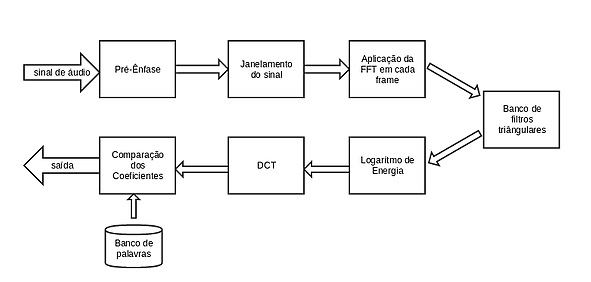
\includegraphics[width=10cm]{img/diaMFCC.jpg} % leia abaixo
\caption{Etapas para extração de coeficientes MFCC.}
\label{fig:diaMFCC}
\end{figure}

O sinal recebido deve passar pelo pré-processamento para reduzir as interferências externas do sinal e ressaltar as informações úteis. Durante a etapa de pré-ênfase o sinal é normalizado. A normalização da amplitude do sinal garante que sons em diferentes alturas sejam processados igualmente. Os períodos de silêncio do sinal são retirados para que apenas dados importantes sejam armazenados.
\begin{itemize}
 \item Após a etapa de pré-ênfase é realizado o janelamento do sinal, ou seja, o sinal é dividido em frames. É aplicada uma janela de Hamming para atenuar as descontinuidades causadas no início e final de cada frame.  A próxima etapa é a aplicação da Transformada Rápida de Fourier (FFT - do inglês \textit{fast fourier transform}) no sinal. A equação \ref{eqima} para obter a potência espectral.
\begin{equation}
\label{eqima}
S[k] = |X[k]|^2 = (real(X[k]))^2 +  (imaginaria(X[k]))^2
\end{equation}
 \item A FFT transforma um sinal do domínio do tempo para um do domínio da frequência.  A  Transformada Discreta de Fourier (DFT - do inglês \textit{discret fourier transform}) possui complexidade $O(n^2)$ e a FFT possui complexidade $O(n log n)$, por este motivo a FFT é usada em aplicações computacionais. A próxima etapa é a aplicação do banco de filtros triângulares, estes exigem uma explicação mais detalhada de como foram feitos. Esta explicação é feita em detalhes na seção \ref{sec:filt_tri}.
 \end{itemize}

\section{Filtros Digitais}
\label{sec:filt:tri}
\quad Filtros digitais são usados para separar os sinais.  Para o processamento de áudio são aplicados os filtros no domínio da frequência, estes filtros selecionam certas regiões  no espectro, bloqueando as demais \cite{sig}. Aplicar diferentes filtros para o sinal de voz implica em diferentes técnicas entre elas, \textit{PNCC, PLP}. Em \cite{mello}, e em \cite{pucpncc}, é possível encontrar uma descrição mais detalhada para descritores de voz. Neste trabalho foi utilizado os filtros triângulares que estão diretamente realcionados a escala \textit{mel}, essa é explicada na seção seguinte. 

\subsection{Escala Mel}
\label{sec:mel}
\quad Em 1937 Stanley Smithy Stevens, John Volkman e Edwin Newmann propuseram o uso de uma variável psicoacústica chamada  \textbf {pitch}  para a criação de uma escala musical perceptual de tons em intervalos igualmente espaçados, chamada escala  \textit {mel}. A frequência ouvida pelo sistema auditivo humano é subjetiva e varia de acordo com cada indivíduo. Esta impressão subjetiva de frequência é a sensação subjetiva da intensidade ou a amplitude de um som. A escala \textit{mel} é uma escala de pitches julgados pelos ouvintes como sendo igual em distância um do outro. O ponto de referência entre esta escala e a medição de freqüência normal é definida  igualando um tom de 1000 Hz , 40 dB acima do limiar do ouvinte , com um pitch de 1000 \textit{mels}. Abaixo de cerca de 500 Hz as escalas de \textit{mel} e Hertz coincidem, acima disso intervalos cada vez maiores são julgados por ouvintes para produzir iteração igual aos pitches. A escala \textit{mel} é baseada em um mapeamento entre a frequência real e o pitch aparentemente percebido do sistema auditivo humano. Para converter uma frequência em escala \textit{mel} aplica-se a equação \ref{melscale}, onde $f$ é frequência.
\begin{equation}
\label{melscale}
M(f) = 1125 ln(1 + \frac{f}{700})
\end{equation}

\subsection{Filtros Triângulares}
\label{sec:filt_tri}
A percepção humana de algumas frequências de sons complexos não podem ser individualmente dentro de certas bandas, quando uma dessas componentes cai fora da banda, chamada de banda crítica, ela pode ser identificada. Isto ocorre porque a percepção de uma frequência particular pelo sistema auditivo, por exemplo $f_0$, é influenciada pela energia da banda crítica das frequências em torno de $f_0$. O valor dessa banda varia nominalmente de $10 \%$ a $20 \%$ da frequência central do som, começando em torno de $100 Hz$ para frequências abaixo de $1 kHz$ e aumentando em escala logarítmica acima disso. Com base nestes fenômenos utiliza-se o logarítmo da energia total das bandas críticas em torno das frequências mel. A aproximação utilizada para este cálculo é a utilização de um banco de filtros espaçados uniformemente na escala mel, o banco de filtros triangulares. Os filtros \textit{mel} são definidos de acordo com a função \ref{filtro}.
\begin{equation}
\label{filtro}
%\begin{displaymath}
H_m[k] = \left\{\begin{array}{ll}
0 & k < k[m-1]\\
\displaystyle \frac{2(k-k[m-1])}{(k[m+1]-k[m-1])(k[m]-k[m-1])}, & k[m-1] \leq k \leq k[m] \\
\displaystyle \frac{2(k[m+1]-k)}{(k[m+1]-k[m-1])(k[m+1]-k[m])}, & k[m] \leq k \leq k[m+1] \\
0 & k > k[m+1]\end{array} \right.
%\end{displaymath}
\end{equation}
 Onde:
$M$ = números de filtros, $m$ = número do filtro, tal que $1 \leq m \leq M$ e $f(m)$ = frequência central de cada filtro.\\

A Figura \ref{fig:filtro} mostra o banco de filtros usados na técnica MFCC. Cada filtro calcula a média do espectro em torno de um espectro central. Quanto maior a frequência, maior é a largura da banda.

\begin{figure}[H]
\centering % para centralizarmos a figura
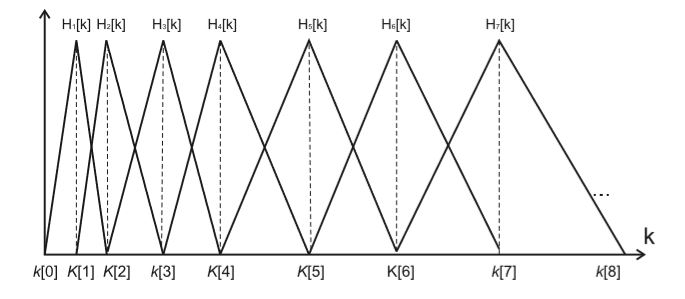
\includegraphics[width=10cm]{img/filtrotriangular.jpg} % leia abaixo
\caption{Banco de filtros triângulares MFCC. \textit{fonte: \cite{pucpncc}}}
\label{fig:filtro}
\end{figure}

Para determinar matematicamente os segmentos, parte-se da frequência extremas $f_l$ e $f_h$ que são as frequências de corte do banco de filtros em Hz. Esses valores são usados para dividir o intervalo em $B+1$ partes iguais. Para obter os valores em Hz, basta aplicar a função inversa \ref{inversa}.

\begin{equation}
\label{inversa}
k[m] = \big( \frac{N}{F_s}\big) Mel^{-1} \big(Mel(f_l) + m \frac{Mel(f_h)- Mel(f_l)}{M+1}\big)
\end{equation}

onde $F_s$ é a frequência de amostragem em Hz, M é o número de filtros e N o número de amostras da FFT. $k[m]$ são as frequências digitais e $Mel^{-1}$ determina a largura do banco de filtros e é dado por
\begin{equation}
Mel^{-1}(m) = 700(e^{\frac{m}{1125}} - 1)
\end{equation}



Em seguida, obtém-se a log-energia da saída de cada um dos filtros \textit{mel}. Por fim os coeficientes MFCC são obtidos aplicando a  Transformada Discreta de Cosseno (DCT - do inglês \textit{discret cosine transform}) ao logarítmo dos coeficientes de energia obtidos no passo anterior.





























